\documentclass[twoside,openright]{uva-bachelor-thesis}

\usepackage{emptypage} % removes page numbers on empty twoside pages

% Fonts and input encoding
\usepackage[utf8]{inputenc}
\usepackage{ae,aecompl}
\usepackage{sourcecodepro}
\usepackage[T1]{fontenc}

% Multiline comments
\usepackage{verbatim}

% Random text
\usepackage{lipsum}
\setlipsumdefault{131}

% Bibliography
\usepackage[square,numbers]{natbib}
\usepackage[nottoc,numbib]{tocbibind}
\renewcommand\bibname{References}

% Footnotes in tables
\usepackage{footnote}

% Colors
\usepackage{xcolor}

% Figures and graphics
\usepackage{graphicx}
\usepackage{epstopdf}
\usepackage{pgfplots} % plotting
\usetikzlibrary{patterns}
\pgfplotsset{width=7cm,compat=1.12}

% References
\usepackage{hyperref}
\hypersetup{pdfborder={0 0 0}} % remove borders around PDF links
\usepackage[noabbrev]{cleveref}

% Remove leading paragraph indent
\usepackage{parskip}
\setlength{\parindent}{0pt}
\setlength{\parskip}{1.3ex plus 0.5ex minus 0.3ex}

% Captions
\usepackage[format=plain,labelfont={sf,bf,up},textfont={it,sf}]{caption}
\usepackage{subfig}

% Minted setup.
\usepackage[chapter,newfloat]{minted}

\definecolor{mintedbackground}{rgb}{0.98,0.98,0.98}
\definecolor{mintedframecol}{rgb}{0.75,0.75,0.75}
\setminted{
	autogobble=true,
	breakbytoken=true,
	breaklines=true,
	escapeinside=\#\%,
	fontsize=\scriptsize,
	tabsize=4,
	baselinestretch=1.2,
	frame=none,
	framerule=0.4pt,
	framesep=3mm,
	rulecolor=\color{mintedframecol},
	numberblanklines=true,
	numbersep=2pt,
	xleftmargin=0pt,
	style=manni
}
\setminted[xml]{
	style=murphy
}

% Use line no's with [frame=leftline,linenos]
\newminted{c}{}
\newminted{xml}{}
\newminted{csharp}{}
\newmintedfile{c}{}
\newmintedfile{xml}{}
\newmintedfile{csharp}{}

% Colorbox.
\usepackage[skins]{tcolorbox}
\tcbuselibrary{raster}
\tcbset{
	enhanced,
	label type=listing,
	fonttitle=\sffamily,
	colback=mintedbackground, colbacktitle=mintedbackground, coltitle=darkgray, 
	arc=0pt,outer arc=0pt, 
	boxrule=0mm, 
	toptitle=2mm, bottomtitle=1mm,
	titlerule=1pt, colframe=gray, titlerule style={mintedbackground, dashed} 
}

% Usage: \begin{codebox}[label=...,other options]{Title} contents from minted \end{codebox}
\newtcolorbox[use counter=listing,number within=chapter]{codebox}[2][] {
	title={\textbf{Listing \thetcbcounter}: \textit{#2}},
	#1
}
\newtcolorbox{codespan}{
	toptitle=0mm,
	bottomtitle=0mm,
}

% To remove
\newcommand{\includecode}[3]{}
\newcommand{\includexml}[3]{}

% Inline formating - could be done by mint
\usepackage{xspace}
\newcommand{\file}[1]{\texttt{#1}}
\newcommand{\code}[1]{\texttt{\footnotesize#1}}
\newcommand{\cs}{C\texttt{\#}\xspace}

% Research questions
\newcommand\researchquestionformat[1]{\begin{quote}#1\end{quote}}
\newcommand\firstquestion{\researchquestionformat{Does the framework offer features which a modern OO-language provides for free?}}
\newcommand\secondquestion{\researchquestionformat{How could a framework of similar purpose be implemented in \cs?}}
\newcommand\thirdquestion{\researchquestionformat{How do the approaches compare in terms of usability and maintainability?}}

\title{An object-oriented \\implementation of the CiviC compiler framework}
\author{Floris den Heijer\\5873355}
\supervisors{dr. C. Grelck}
\signedby{}

\begin{document}
\maketitle
\begin{abstract}
	\lipsum
\end{abstract}

\tableofcontents


\chapter{Introduction}
	\section{Problem Statement}
		Computer Science undergraduates at the University of Amsterdam have the option to learn the essentials of compiler construction by taking an 8-week course where the main deliverable is a working compiler for a model programming language named CiviC, or \emph{Civilized C}. This language exhibits characteristic features of structured imperative programming languages and is designed in a way to be sufficiently restricted in size and complexity for the course. Students may optionally implement more advanced features such as arrays and nested functions for extra credits. Construction is assisted by a framework which offers structured approach to compiler development.
		
		The framework functions as a template, providing the necessary infrastructure and hooks for further development. It is written in C, a language most students are familiar with. It can be considered succesful, as nearly all students deliver working compilers with it and the course is received well. A recurrent problem during the first weeks of the course is the difficulty in getting up to speed with the framework. This is in part due to a lack of documentation, but it is suspected language plays a role as well. 
		
		A recent large-scale study found that features in a programming language considered most important were object inheritance, classes, exceptions and garbage collection\cite{Meyerovich2013}. Although the study might be biased towards users of dynamic programming languages, over 60\% of respondants found static typing to be of at least medium importance. The framework's language (C) delivers little to none of these features. While it is statically typed, it is generally considered a `weakly'-typed language compared to modern object-oriented languages. Languages such as Java and \cs have more rigorous type checking and provide mechanisms to catch runtime violations of the type system. Static types have been demonstrated to serve as a source of documentation and may help programmers to use a new set of classes\cite{Hanenberg2014}.
		
		While C is unrivalled for it's high-speed, is it the right choice for the CiviC compiler framework? Does the framework utilize techniques which are only possible in C? Are there features made obsolete by simply using a modern statically-typed and object-oriented language? This paper will present an in-depth analysis of the CiviC compiler framework, documenting it's architecture, workflow and implementation. A new framework with the same goals as the existing one will be presented, but written in \cs. Both approaches are rated on usability and maintainability, and the  question \emph{which is better} is discussed.
		
			
	\section{Context}
		\begin{itemize}
			\item Discuss course and objectives
			\item Explain setting of framework
			\item Explain purpose of framework in more detail
			\item Compare against other frameworks
		\end{itemize}
	
		The CiviC compiler framework is used in a strictly educational setting and succesfully assists students in creating a  fully functional compiler for the CiviC model language.  and are there any comparable alternatives?
		
		The course is structured to gradually walks students through all stages of compiler design. The first weeks are centered around frontend stages, such as AST design, scanning, parsing, semantic analysis and type checking. Only in the last few weeks are students introduced to the language they are compiling to, which is an assembly language for the CiviC-VM. 
		
		and very little attention is spent on heavy backend stages like code generation and optimization. This focus is not a bad thing, as the approach clearly works, delivering passing students with functional compilers every year.
				
		As for other compiler frameworks, there aren't many general purpose versions about. The most well-known example might be the LLVM compiler infrastructure project\cite{lattner2002llvm}, though it primarily fulfills a backend role by providing the specification for it's intermediate representation (IR) and a suite of backends targetting nearly every instruction set. Frontends targetting its IR are written by the community for a variety of languages, including Haskell and Python. Most other frameworks fill specific hardware niches such as GPGPU transpilers or optimizers for embedded IPC's.
		
		There is one framework which stands out: Polyglot\cite{polyglot}. It has been primarily developed to assist in creating compilers for languages like Java, Java language extensions, implementations of of domain specific languages and for ''\ldots simplified versions of Java for pedagogical use''. It's architecture and design choices will be considered in future chapters.
		
		
	\section{Research Questions}
		The main questsions of this project are:
		\firstquestion
		\secondquestion
		\thirdquestion
		
		Under `framework of similar purpose', a framework is understood which:
		\begin{enumerate}
			\item Can be used to construct a CiviC compiler during the 8-week course
			\item Provides a structured approach to compiler construction
		\end{enumerate}

	
	\section{Research Approach}
		To answer \firstquestion an in-depth of the CiviC framework will be given documenting it's architecture, workflow and technical underpinnings. Combined with knowledge of \cs, the question can be objectively answered.
		
		To answer \secondquestion the design process of such a framework will be documented. Specifically, the topic of type-safety and it's effect on key framework features will be discussed.
		
		To answer \thirdquestion it is necessary to define usability and maintainability. While methods exist which quantify usability and maintainability to some degree, they are geared mostly towards rating enterprise software or based on large-scale surveys. The CiviC framework and it's userbase are too small for these methods, however it's size does warrant a more subjective approach.
		
		Usability will be determined by comparing:
		\paragraph{Clarity of user code}
			Reference code will be judged primarily on conciseness. There are obviously major differences between C and \cs, but it might be precisely these differences which makes one framework more accessible.
		
		\paragraph{Transparency of framework}
			Without detailled knowledge of the framework, how easy is it to understand how it how it functions and how user code fits in? Although it is not necessary to understand framework mechanisms in detail, users should have a rough idea of how it helps them; if not for debugging then for extensibility.
			
		Maintainability is primarily relevant for those maintaining the framework, as most CiviC compilers will never be used outside of the  course. A rough measure can by established by comparing the size of the code base.
		
	
	\section{Scope And Limitations}
		This paper is limited to the compiler framework of the CiviC toolchain and will not review the applicability of the the Civic VM and assembler. Teaching objectives or the suitability of alternative target languages such as LLVM, CIL or Java bytecode are also also outside of the scope for this project.
			


\chapter{Analysis Of Civic Framework}
\label{analysis}
	This chapter will provide an in-depth review of the existing framework, detailing it's architecture, workflow and technical implementation. The chapter concludes with a discussion on the 
				
	\section{Architecture}
		On a high level the framework aims to provide a structured approach for phase-based transformations on a language agnostic AST or \emph{abstract syntax tree}. Central to the framework is a specification of the AST and a code generator which produces interaction code and traversal control mechanisms. Interaction code here means an interface through which AST nodes can be created or modified, and composed into a tree. Manipulation of a tree is achieved through \emph{traversals}, which target specific set of nodes and specify code to be executed for each node, much like the visitor pattern introduced in the next chapter. The framework recognizes distinct \emph{phases} of compilation, such as semantic analysis or code generation, and provides a way to group related transformations and execute them sequentially.
				
		\begin{figure}[H]
			\centering
			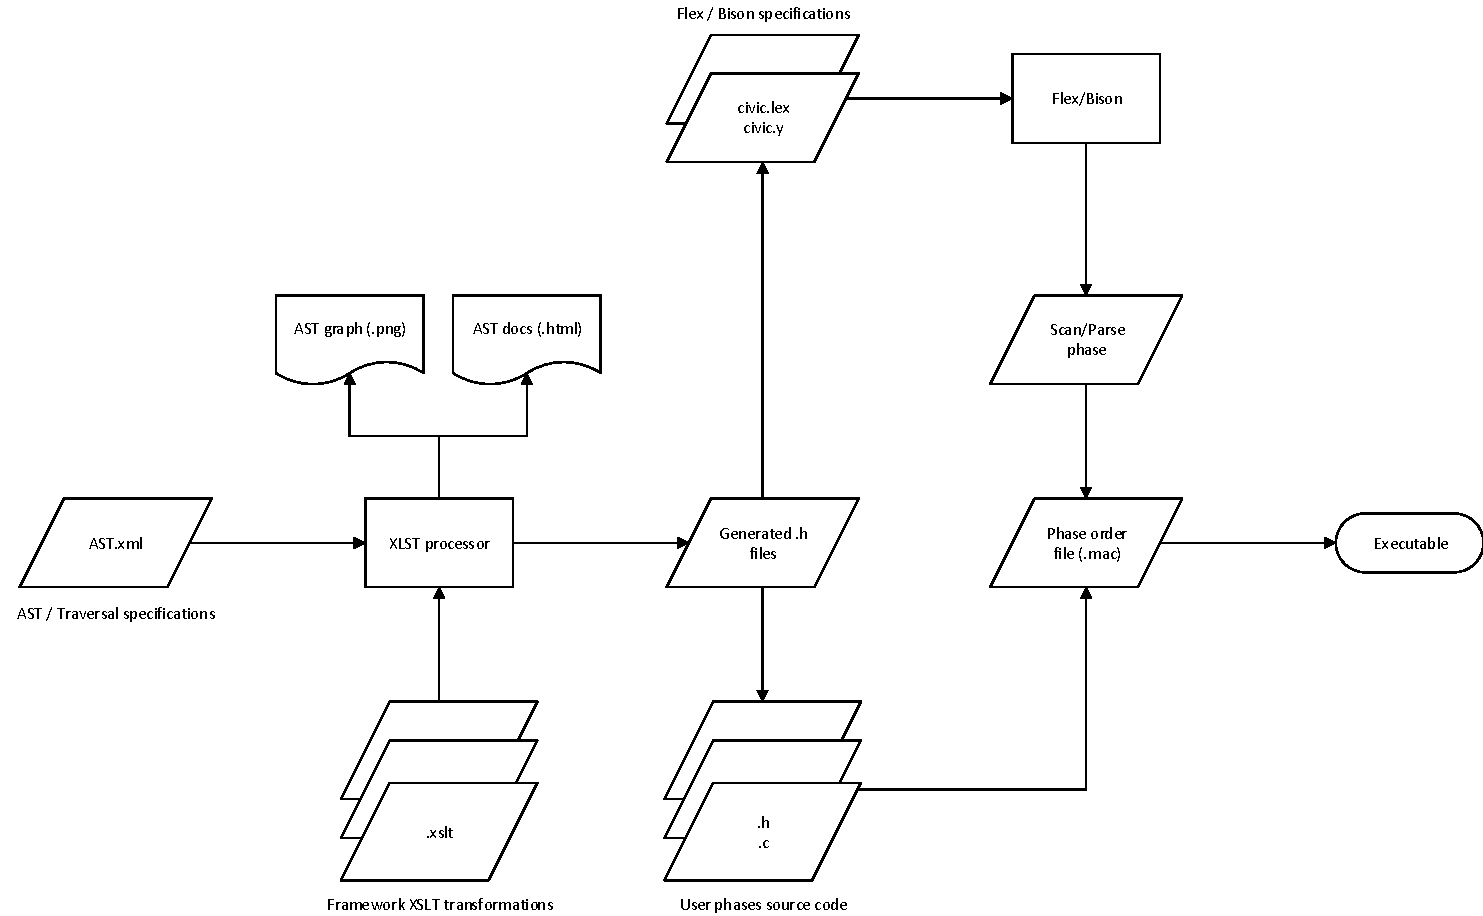
\includegraphics[width=0.95\textwidth]{figures/architecture/overview.pdf}
			\caption{Schematic overview of the Civic framework}
			\label{build-dep}
		\end{figure}
		
		The framework is written in C and XLST and runs on most *nix distributions, provided they support the required packages\footnote{gcc, gzip, flex, bison, xsltproc, dot, indent}. A schematic overview of the architecture is presented in \cref{build-dep}. The framework relies on an XSLT processor to transform a specification of the AST and traverals into C header and source files which can be used by the rest of the compiler. This process is triggered on each build and replaces key files if the specifications are altered.
		
		
	\section{Workflow}
	\label{c-workflow}
		The framework enforces a specific workflow and code organization structure. It presents the process of compilation as a pipeline of phases, each phase consisting of one or more traversals. Users can modify or expand the pipeline by introducing new phases and traversals, but are bound by this structured approach. Configuration of the pipeline is possible through code and supported by C macro's further explained in the next section. Seperated from code are the specification of the AST and traversal definitions. 
		
		This workflow directs user code largely to:	
		\begin{enumerate}
			\item Specification of AST and traversals (\code{AST.xml})
			\item Traversal header and implementation files (user directory with \code{*.c, *.h} files)
			\item Pipeline configuration file (\code{phase.mac})
		\end{enumerate}
		
		As each compiler requires scanning and parsing, a phase invoking the Flex scanner generator and Bison parser generator are provided by default. While strictly part of bootstrapping code, most users will work with these tools, adding to the above list:
		\begin{enumerate}
			\setcounter{enumi}{3}
			\item Lex configuration for Flex (\code{civic.l})
			\item YACC configuration for Bison (\code{civic.y})
		\end{enumerate}
		
		Changes to the AST or the addition of a new traversal are propagated by building the compiler. The build process produces updated integration code as well as documentation on the AST in two forms: 1) as an HTML document detailing every node and it's children, and 2) as an image depicting the AST graphically, with lines connecting nodes where applicable.
		
		Debugging is assisted through command line arguments which can specify to only compile up to a certain point. The command line also allows configuration of tracer options, which - assuming the user supplemented their code with the required statements - enables detailed output of the callstack.
	
		
	\section{Technical Implementation}
		The most defining characteristic of the framework is the abstraction layer over the AST and traversal mechanisms. To better understand this layer, this section will detail the internal representation of nodes, traversals and phases and discuss the role of code generation. \emph{This section assumes knowledge of the C programming language.}
				
		\subsection{Abstract Syntax Tree}
		\label{c-ast}
			\begin{codebox}[label=xml-node-structure]{Template for specification of a node}
				\xmlfile{samples/node_structure.xml}
			\end{codebox}
			
			\begin{codebox}[label=c-node-structure]{Internal structure of a node}
				\cfile{samples/c_node_structure.c}
			\end{codebox}
			
			Nodes in the AST are defined as a \code{<node>} XML element under the \code{<syntaxtree>} inside the \code{AST.xml} specification file. Every node has a name, and optionally a list of named child nodes (or \emph{sons}) and attributes, following the template shown in \cref{xml-node-structure}. The difference between an attribute and a child node is that child nodes can be traversed, whereas attributes are simple properties, though they might in fact reference other nodes. The \code{<targets>} element inside either a child or attribute element is among other things used to declare a property as mandatory, this is further explained in \cref{tree-validation}.
			
			Internally, nodes are represented by the \code{NODE} structure shown in \cref{c-node-structure}. This structure holds the type of the node as an \code{enum} and references to two union structures representing applicable child nodes and attributes. These structures are generated and union'ed based on the XML specification, which translates a \code{<son>} element to a \code{node*} member of the former and an \code{<attribute>} element to a typed member of the latter. The C-type used for members of the attribute structure comes from a mapping section in the specification.
			
			Besides one being traversible, child nodes and attributes are accessed the same way through generated macro's. These macro's primarily exist to avoid manually selecting which union struct variable should be accessed. A side effect is that it also hides which properties are children and which are attributes, and it implies an attribute cannot have the same name as a child node. Access macro's \emph{do not} ensure they are used on the correct node by validating the node type, as they are used both as a setter on the left-hand side and a getter on the right-hand side, and assignment to condidionals is illegal in C.
			
			Creating nodes is a straightforward process as allocation code for each node is generated from the specification. Every node has a create function, which accepts references to child nodes as well as attributes marked mandatory. Free-ing nodes is a recursive operation which requires a traversal and is covered in the next section.
			
		\subsection{Traversals}
		\label{c-trav}
			\begin{codebox}[label=xml-trav-structure]{Template for specification of a traversal}
				\xmlfile{samples/trav_structure.xml}
			\end{codebox}
									
			Traversals do not have a single, well-defined structure but rather translate into control flow statements and traverse tables. Every traversal must be declared in the \code{AST.xml} file as a child of the \code{<phases>} element and must adhere to the template presented in \cref{xml-trav-structure}. They require a unique prefix, a friendly name, mode of operation and header file with handler declarations.
			
			All handlers have the same function signature: passed in are pointers to an input node and info structure, a pointer to the output node is returned. The info structure may be defined by the traversal and can be used to share state between traversal methods. Handler declarations are not generated and must be declared by hand.
			
			Two operation modes are supported: 1) user mode and 2) child mode. User mode traversals are required to implement handlers for every node type in the AST, child mode requires only handlers for a set of nodes specified in the \code{<travuser>} element. In child mode, every node not in that list is handled by a catch-all function which automatically traverses child until one a node is found for which a handler is registered.
			
			To initiate a traversal, users must push it's identifier onto the stack and invoke the \code{TRAVdo} or \code{TRAVopt} traverse functions\footnote{TRAVdo does not allow traversal of a null argument, the TRAVopt function only invokes TRAVdo on a not-null argument.}. These functions have the same signature as handlers and should in fact be seen as a smart wrapper around them, choosing the correct handler based on node type and active traversal. Traversals may be nested by pushing another traversal onto the stack and calling the traverse function again, though not all traversals support this kind of initiation. More specifically, only traverals devoid of an info structure support this approach, as the allocation and de-allocation of this structure is always static to the owning traversal. Passing parameters to nested traversals would require a seperate entry point with accompanying parameters. Initiation of a traversal is illustrated in \cref{c-trav-example}.
			
			Once a node is passed into the main traversal function, a lookup on node type to the function table for the active traversal will return a handler for that node. The traverse tables are generated from specification, with user mode requiring function references for all node types, and child mode filling in the gaps with the \code{TRAVsons} function. This is the catch-all automatic traversal function which uses a large switch statement on node type to invoke the traversal function on every child node, the result of which is put back to the property. Once all children are traversed the input node is passed back to the original caller. An excerpt of a generated \code{TRAVsons} function is shown in \cref{c-trav-sons}. 
			
			\begin{codebox}[label=c-trav-example]{Example of traversal invocation}
				\cfile{samples/c_init_trav.c}
			\end{codebox}
			
			\begin{codebox}[label=c-trav-sons]{Part of the generated TRAVsons catch-all function}
				\cfile{samples/c_trav_sons.c}
			\end{codebox}
			
			Three important traversals are generated on every build:
			\begin{enumerate}
				\item Copy traversal, which creates a deep copy of the structure (child nodes) and a shallow copy of all attributes
				\item Free traversal, which de-allocates a tree and - if applicable - it's attributes
				\item Check traversal, responsible for validating AST integrity
			\end{enumerate}
			
			Attributes are copied and freed based on their specification in the previously mentioned \code{<asttypes>} element, which identifies three situations: 1) node references, 2) strings and 3) value types and other references. Node references as attributes are not followed and only the reference is copied, freeing a node attribute only nulls the reference but leaves the structure intact. Strings are copied and freed using string library functions, and all other value and reference types are copied using straight C assignment. The check traversal will be discussed in \cref{tree-validation}.
					
		\subsection{Phases}
		\label{old-phases}
			As briefly described in \cref{c-workflow}, configuration of the phase pipeline is done through code with the assistance of helper macro's. Configuration is achieved through the \code{phase.mac} file, where users can define a phase as a logical distinction or practical grouping of traversals. A friendly name can be assigned to each phase, which, in debug mode, is written to \code{stdout}. In addition each phase is assigned a unique identifier which can be used for validation as detailed in the next section. Traversals in a phase must also specify a friendly name for the same debugging purpose as their parents and more importantly the name of the entry point to the traversal. Traversal entry points are nearly identical in signature to handlers, except they do not accept an info structure as an argument. Entry points usually allocate an info structure, though this may be ommitted, and push a traversal onto the stack, much like \cref{c-trav-example}.
			
			On compilation, macro's in the \code{phase.mac} file are resolved and the traversals are flattened into a sequence and wired up to feed the result of one traversal into the next. Debugging code which allows command line arguments to specify which phases should run is also integrated. At runtime the pipeline can be conditionally halted or aborted by the user during transformation with the \code{CTI*}\footnote{CTIterminateCompilation, CTIwarn, CTIabort, CTIerror, CTIerrorContinued, etc.} range of functions.
		
		\subsection{Tree Validation}
		\label{tree-validation}
			As explained in section \cref{c-ast} all nodes share the same structure, differing only on node type and which variables of two union structures are used. The nodetype \code{enum} in conjunction with the switching mechanism and access macro's provide the basis for a tagged union construct, though this is not enforced in any way. Thus, semantically all nodes are valid trees, yet most combinations of AST nodes should be recognized as an invalid tree. 
			
			This is where the check traversal mentioned in \cref{c-trav} comes in. This generated phase validates all constraints set in the AST specification and aborts compilation on an invalid tree. Constraints can be set in the \code{<targets>} element optionally placed inside a child declaration or type element of an attribute (see \cref{xml-node-structure}). Both child node and attribute properties support the \emph{mandatory} constraint, which invalidates the tree if found empty. 
			
			While a type definition is always required on an attribute, child nodes allow any node unless specified otherwise. The \code{<node name="..."/>} element signals the check traversals that there is only one node type valid for the child position. Often this is not sufficient, as children operate may operate on \emph{sets} of nodes. An example of this is any expression language, where an operator may act on any expression, itself included. The framework allows flexibility in the specification of valid child nodes through \emph{nodesets}, which are defined as children of the \code{<nodesets>} element. A nodeset has a name and list of named nodes which belong to the set. Nodesets may not be nested.
			
			Constraints may only be valid during or after certain phases. The framework supports this by allowing multiple \code{<target>} elements for properties. Users can specify a range of phases to which the constraint applies, using the phase identifier from the last section. The example in \cref{c-targets} shows a hypothetical node which during early compilation phases may contain any node from the expression set, while in later phases the node must contain a reference to an integer constant node.
			
			\begin{codebox}[label=c-targets]{Phase ranged constraints and targeting of a nodesets}
				\xmlfile{samples/targets.xml}
			\end{codebox}
		
		
	\section{Features Found In OO-Languages}
	\label{oofeatures}
		The framework provides a wide range of features applicable for compiler construction. Some of these features seem at least partially focused around providing a level of type-safety and object-orientation not found in C.
			
		\paragraph{Tagged union}
			Nodes in the framework are represented by the \code{NODE} structure which, depending on node type, holds two other structures with child nodes and attributes. This can be seen as a primitive form of object inheritance, where the node structure functions as an abstract base class and all nodes as concrete implementations. The \code{NODE} struct is abstract because it holds a variable with an enumeration of all possible nodes, which means it's not possible to construct a node from code alone without also modifying that - generated - enum.
			
		\paragraph{Access macros}
			The access macros are obsolete if a node were to be represented as an object, instead of a composition of structures. Although the macros do not check for correct type due to their use on both sides on both sides of an assignment, an OO-language would provide this additional type-safety for free.
			
		\paragraph{Memory management}
			The most obvious feature most modern OO-languages offers is automatic memory management. The \emph{free}-traversal can be removed entirely if a language with garbage collection is used. Similarly, object construction is done on a much higher level.
			
		\paragraph{Validation traversal}
			The \emph{check}-traversal is primarily used to ensure nodes have valid children. If child nodes were to be typed properties of an object, this responsibility is handed to the compiler. The \emph{nodesets} defined by the framework are only used in this context, and offer a limited form of inheritance. Inheritance doesn't allow nodes to belong to multiple nodesets directly, which is allowed by the framework; however the framework doesn't allow nesting of nodesets, which \emph{is} allowed by inheritance. 
			
		\paragraph{Info structure}
			Passed along with every traversal action is a traversal specific \code{INFO} structure, whose sole purpose is the sharing of state between traversal methods. If a traversal were to be seen as a class, this state could be transfered to member variables of the class.
	
	\begin{comment}
	\section{Code Generation From XML}
	\label{sec:old-sec}
			One defining characteristic of the framework is an abstraction layer over the AST and traversal mechanisms. To better understand this layer, this section will first summarize how nodes and traversals are internally represented, then detail how the abstraction assists in this process and conclude with a summation of all parts of the framework affected by the layer.
			
			Nodes are stored as a C-struct containing the type of the node and two structures representing their children and attributes (snippet \ref{old-arch:node}). For each node type there are two data structures with it's specific attributes and references to child nodes, the union of which is refered to in the \code{NODE} struct (snippet \ref{old-arch:union}). Access macro's are created for each attribute and child node as well as (de-)allocation code.

			Traversals do not have a well defined single structure but translate into control flow statements and traverse tables. Users can push a traversal onto the stack and request the start of a traversal (snippet \ref{old-arch:start-trav}), triggering a lookup to a table for the active traversal holding the function which should be called index on node type. By default all child nodes are traversed using a switch statement based on node type (snippet \ref{old-arch:switch-trav}). The \code{INFO} struct passed along provides statefulness to receiving functions, though this is not essential for traversal.
			
			To illustrate the complexity involved, consider the introduction of a new node to the AST. To achieve this, every traverse table must be supplemented, the default traverse function must be updated, two new structures must be added to the node union, allocation and de-allocation routines must be written as well as access macro's and the copy, free and check system traversals must be modified. Besides being tedious, performing these tasks manually introduces a significant risk of error. The framework provides XSLT transformations of a specification to automate most of this process. It takes only a couple of lines of XML to add a node to the AST, and all previously mentioned tasks are automatically executed. This does however mean that the specification forming the abstraction is not isolated from the target language (or leaky). For instance, to define a node with a \code{char*} attribute requires the specification to know about the difference in copying C-strings and integers.
					
			Specifications and accompanying translations are given for:
			\begin{itemize}
				\item Nodes which form the abstract syntax tree, along with their applicable attributes and child nodes
				\item Mapping from friendly attribute names to C-types, and relevant methods used for copying and free-ing
				\item Node constraints on:
				\begin{itemize}
					\item Type: only certain child nodes or attribute are valid
					\item Requirement: attributes or child node must be present
					\item Applicable phase: some attributes are not always required
				\end{itemize}
				\item Traversals, their mode of operation, affected nodes and function prefix
			\end{itemize}
		
	\section{Flexible Traversals}
			Internals of the traversal have been briefly shown in section \ref{sec:old-sec} and will be explained in more detail in this section. 
			
			Traversals are supported in two modes: 1) user mode and 2) child mode. User mode traversals are required to implement handlers for every node type defined in the AST, child mode requires only handlers for a specified list of nodes. Every node which is not on the user specified list is routed instead to a catch-all function which automatically traverses child nodes of the unhandled node. This function is automatically updated when a node is added or removed or a change is made to any of the child node properties.
			
			All traversals are elements in the \code{<phases>} element of the specification document, and must contain a unique identifier, readable short name, operation mode (user or child), associated header file and - depending on the chosen mode - a list of nodes handled by the traversal. When the compiler is built, enumerations of all node and traversal identifiers are generated. All nodes and traversals are assigned a zero-indexed integer to be used as an index. Every traversal adds an array of function pointers to the traverse table. The row is added at the index dictated by the enumeration and the array is indexed by the node index. References to the funtions are constructed by concatenating the traversal identifier with the friendly name of the node. In child mode, unhandled node types are routed to the catch-all function explained in the last paragraph.
			
			Every handler has the same function signature, requiring pointers to a node and an info structure, and returning a pointer to a node which replaces the current node. If a traversal is to be used as an entry point for a sub-phase, it must be added to the \code{phase.mac} file, where an entry point is referenced with the same signature as a handler function: \\
			\code{node *PFXnodeType (node *arg\_node, info *arg\_info)}
						
			The framework maintains a stack of active traversals manipulated with the \code{TRAVpush (id)} and \code{TRAVpop ()} functions. An active traversal can be controlled with the \code{TRAVdo (node*, info*)}, \code{TRAVopt (node*, info*)} and \code{TRAVcont (node*, info*)} functions. All return the result of the traversal of a given subtree, additionally the latter two respectively ignore null node arguments and invoke the catch-all handler.
			
			This approach to traversals encourages users to create small, reusable traversals in similar way the visitor pattern is implemented in an object-oriented language \cite{gof1994}.
			
	\section{Tree Validation}\label{sec:validation}
			As explained in section \ref{sec:old-sec}, nodes all share the same structure. Semantically all node structures are valid trees, yet most combinations of AST nodes should yield an invalid tree. This section briefly explains the validation mechanisms present in the framework.
			
			The first line of defense against illegal node operations is the tagged union implemented for nodes. A tagged union is a structure which can take on different but fixed types \cite{unknown}. An \code{enum} is used to distinguish all different node types and used in the generated traversals to always pick the correct structure when traversing. Unlike functional languages, C provides no compile time checks to enforce the tagged union except for a simple check on the node type. However, access to nodes and traversal mechanisms are largely controlled from generated macro's which do provide a level of security. It must be noted that the macro property accessors do not check the node type, as they are used on both the left- and righthand side of assignments and assignments to conditionals are illegal in C.
			
			The main validation mechanism lies in the 'check' traversal generated from the AST. This traversal walks the AST and ensures that every node has child nodes and attributes of the correct type, and that any attribute or child node marked as mandatory for the current phase is present. The check traversal must be manually added as part of a phase, so invalid trees are still possible during execution of any traversal up to the check. 
		
	\section{Development Environment}
		Todo:
		\begin{itemize}
			\item Error handling
			\item Pre-configured scanner, parser
			\item Debug helpers
			\item Compact base library
		\end{itemize}
	\end{comment}
	
	
\chapter{Re-Design In \cs: Code-First Approach}
	Expanding on \cref{oofeatures}, this chapter documents the design of an object-oriented framework centered around the same principles as the C-based framework. First the choice of \cs is explained, along with a small primer on some of it's unique features. Then, the applicability of an AST abstraction layer as found in the current framework is challenged by developing a model for a type-safe AST. Development and optimization of two type-safe traversal mechanisms is covered next and the chapter concludes with a model for a code configured compiler pipeline and a discussion on representing collections in an AST.
		
		
	\section{\cs Primer And Motivation}
	\label{csprimer}
		When considering imperative programming languages which are statically-typed, object-oriented and have automatic memory management the most obvious candidate would be Java. Most students have experience with Java as it is part of many other courses. So why \cs? This section briefly discusses unique features of \cs and why it is prefered over Java. It also doubles as a primer for readers not accustomed to it.
		
		\paragraph{var keyword}
			Writing staticaly-typed code can be a verbose affair. Initializing a class and assigning it to a variable in Java means typing the class name twice: once for the type of the variable, once for the calling the constructor of the class. This is tedious work and doesn't enhance readability by any stretch of the imagination. \cs 3.0 introduced the \code{var} keyword, which infers the type based on the assignment to it. It can only be used in function scope and requires a direct assignment.
			
			\begin{codespan}
				\begin{csharpcode}
					// Without var:
					SomeExtremelyLongClassName onlyRelevantData = new SomeExtremelyLongClassName();
					foreach (SomeExtremelyLongClassName item in ...)
						...
					
					// With var:
					var onlyRelevantData = new SomeExtremelyLongClassName();
					foreach (var item in ...)
						...
						
					var a = 5.0;        /* equivalent to float a = 5.0; */
					var b = null;       /* illegal, type cannot be infered */
				\end{csharpcode}
			\end{codespan}
			
		\paragraph{Auto-implemented properties}
			Defining publicly variables on a class is `bad-form' in the object-oriented world for many reasons. Exposing a member variable means the declaring class effecively loses control over it as external code can easily set it to \code{null} or a new reference. Control to variables is often wrapped with get/set methods, which return or set the member variable. This also allows code to mark data as read-only by only exposing a getter. In Java these methods must be written by hand, resulting in often tedious work or a task performed by the IDE. \cs 3.0 introduced automatic properties, a compact and flexible way to define a private field and how define it's access logic. Properties can be initialized when constructing a class with an initialization block, eliminating the need for a constructor in most simple objects.
			
			\begin{codespan}
				\begin{csharpcode}
					class Person
					{
						public string Name { get; set; }
						public string NameInCaps
						{
							get { return Name.ToUpper(); }
						}
						
						public int Id { get; private set; }
					}
					
					var peter = new Person
					{
						Name = "Not Peter"
					};
					
					peter.Name = "Peter";                /* sets Name property */
					Console.WriteLine(test.NameInCaps);  /* prints "PETER" */
					peter.Id = 5;                        /* error, id can only be set from private scope */
				\end{csharpcode}
			\end{codespan}
						
		\paragraph{Dynamic cast}
			The \code{dynamic} keyword introduced in \cs 4.0 is similar to the \code{var} keyword introduced above, except instead of defering resolution to compile time, the type is resolved \emph{at runtime}. It allows constructs normally found in dynamic languages, such as duck typing, though this is of little use to this project. Objects can also be cast to the dynamic type, which extends \cs further with dynamic dispatch. In the example below the \cs's single-dispatch and dynamic dispatch are demonstrated.
			
			\begin{codespan}
				\begin{csharpcode}
					void PrintIt(Object o)
					{
						Console.WriteLine("It's an object!");
					}
					
					void PrintIt(string s)
					{
						Console.WriteLine("It's a string!");
					}
					
					object test = "Hello there";
					PrintIt(test);               /* prints "It's an object!" */
					PrintIt((dynamic) test);     /* prints "It's a string!" */
				\end{csharpcode}
			\end{codespan}
			
		\paragraph{Anonymous types}
			While Java allows anonymous classes but still requires the definition of a public interface these classes adhere to. \cs 3.0 provides a mechanism for the construction of classes which encapsulate read-only properties without the definition of a type. Why this is so useful is demonstrated later, but for now it's just a convenient way to pack properties in a type-safe manner.
			
			\begin{codespan}
				\begin{csharpcode}
					var p = new { Name = "Peter", Age = 25 };
					Console.WriteLine(p.Name);       /* prints "Peter" */
					Console.WriteLine(p.Age * 2);    /* prints 50 */
				\end{csharpcode}
			\end{codespan}
								
		\paragraph{True generics}
			Though \cs and Java both have generics, there is a big difference in how they are implemented. Java generics use type erasure, which means a generic class is not actually generic, but operates on Objects uses casts to achieve type-safety. In effect they are a compile time construct and not available at runtime, which has significant implications on reflection and constraints. Generics in \cs are supported at byte-code level by the \emph{Common Language Runtime} or CLR, which allows deep type-checking and more detailled reflection\cite{website:java-generics}.
			
			Generic constraints in \cs can specify a type argument to adhere to a specific inheritance relationship, such as a mandatory base class or other generic parameter. They can also specify a parameter to be a value-type or reference type\footnote{The CLR categorizes types in these two classes; all primitives such as \emph{int}'s, \emph{float}'s and \emph{struct}'s are value-types and everything derived from \emph{Object} is a reference type, such as \emph{class}'es but also \emph{string}.}, or that the reference type supports parameterless construction. Generics are supported on classes, interfaces, delegates and methods. Interfaces and delegates additionally support covariance and contravariance in their generic type arguments with respectively the \code{out} and \code{in} keywords. A short example is given below.
			
			\begin{codespan}
				\begin{csharpcode}
					class Animal { }
					class Fish : Animal { }
					class Salmon : Fish { }
					
					class Bear : Animal, IEatsAnimal<Fish> { }
					
					interface IEatsAnimal<in T>
						where T : Animal
					{
					}
					
					void FeedAnimal<TPred,TPrey>(TPred who, TPrey food)
						where TPrey : Animal
						where TPred : IEatsAnimal<TPrey>
					{
					}
					
					var someAnimal = new Animal();
					var salmon = new Salmon();
					var bear = new Bear();
					
					FeedAnimal(bear, salmon);      /* compiles, as salmon is convertible to fish */
					FeedAnimal(bear, someAnimal);  /* fails to compile, someAnimal is not a fish */
				\end{csharpcode}
			\end{codespan}
			
		\paragraph{Lambda expressions}
			Lambda expressions are inline, local functions which can be passed as a function argument or returned as the value of a function call. They come in two variants: expression lambda's and statement lambda's. Both follow a similar construct, with a definition of input parameters enclosed with parentheses, followed by the \code{=>} lambda operator, followed by either an expression or a series of statements enclosed with braces.
			
			They are different from \emph{delegates}, in that a delegate represents a method's \emph{type} by defining it's parameter list and return type as well as reference to the method. In a way they are a type-safe variant of function pointers in C. Lambda's can be used to \emph{create} delegates as well as expression trees, though expression trees won't be covered in detail. A lambda can is convertible to an expression tree and can be compiled back to a delegate, allowing dynamic modification of executable code.
			
			Lambda's can be assigned to any delegate, but not to an implicit local variable (i.e. \code{var}). The .NET framework defines a number of generic delegates specifically for use as anonymous delegates. A function with a \code{void} return type and no arguments is represented by the \code{Action} delegate, a \code{void} function with one argument by the \code{Action<T>} delegate, etc. Functions with non-void return types are represented by the \code{Func<TResult>} delegate when they take no arguments, \code{Func<T, TResult>} if they have one argument, etc.
			
			\begin{codespan}
				\begin{csharpcode}
					Func<int, int, int> add = (a, b) => a + b;
					int result = add(2,5);     /* result = 7 */
					
					Action<string> print = (s) => Console.WriteLine(s);
					print("Hello");            /* prints "Hello" */
				\end{csharpcode}
			\end{codespan}
			
		\paragraph{Extension methods}
			Extension methods are in essence syntactic sugar for static methods, allowing them to be accessed `as-if' they were instance methods. It is mainly a tool to increase readability of code when consuming classes from another project. Extension methods cannot access internal class variables and must be declared on a static class. The type they `extend' must be their first parameter and must be preceeded by the \code{this} keyword, somewhat similar to how class functions are defined in Python.
			
			\begin{codespan}
				\begin{csharpcode}
					static class Extensions
					{
						public static void SayHello(this Ext.Object obj)
						{
							Console.WriteLine("External object says hello");
						}
					}
					
					var externalObject = new Ext.Object();
					externalObject.SayHello();    /* prints "External object says hello" */
										
				\end{csharpcode}
			\end{codespan}
			
		\paragraph{LINQ}
			LINQ, or \emph{Language Integrated Query} is a set of extension methods which operate on the .NET collection interfaces, providing native data querying capabilities to \cs\cite{website:msdn-reflection}. LINQ calls can be chained in a \emph{fluent-style}, making them highly integratable. They use many of the techniques described above, building on extension methods, lambda expressions, generic delegates and anonymous types. It provides a default implementation on all CLR\footnote{Common Language Runtime} objects, but allows data providers to implement part or the full range of methods. This has resulted in providers for SQL, XML, JSON, expressions, and many more.
			
			An example of a LINQ interface is \code{IEnumerable<T>} which defines a class can be enumerated to return objects of type \code{T}. By using extension methods which operate on the enumerable interface, a class doesn't have to implement anything more than the basic functionality it provides. The most frequently used LINQ methods are documented in the next sample. All \cs .NET collection classes like \code{List<T>} and \code{Dictionary<TKey, TValue>} implement the LINQ interfaces. They integrate very well with anonymous classes.
			
			\begin{codespan}
				\begin{csharpcode}
					var ints = new List<int> { 1, 2, 3, 4, 5, -2, -3, 0, 0 };
					
					// Projection:
					//   .Select(Func<int, TResult> func) -> IEnumerable<TResult>
					ints.Select(i => i*2);          /* returns enumerable of 2*i */
					
					// List, array, dictionary conversion
					//   .ToList(), .ToArray()
					//   .ToDictionary(Func<int, TResult> key) -> IDictionary<TResult, TKey>
					ints.ToArray();                 /* returns array of ints */
					
					// Counting:
					//   .Count(), .Count(Func<int, bool> predicate)
					ints.Count(i => i % 2 == 0);    /* equals 4 */
					
					// Tests:
					//   .All(int => bool), .Any(int => bool)
					ints.Any(i => i > 10);          /* returns false */
					
					// And many more, some shown here:
					var sum = ints
						.Distinct()          /* filter non-unique elements */
						.GroupBy(i => i%0)   /* group on even/uneven */
						.SelectMany(g => g)  /* flatten nested collection */
						.OrderBy(i => i)     /* ordering */
						.Where(i => i > 10)  /* filtering */
						.Sum(i => i*2);      /* summation */
				\end{csharpcode}
			\end{codespan}
			
	
	\section{Type-Safe AST}
	\label{type-safe-ast}
		Working with a strongly typed OO-language grants the ability to model AST nodes in greater detail than before possible. The most intuitive way is to represent different types of node with distinct classes. All nodes derive at some point from an abstract base class, though intermediate classes can also be created to allow for hierarchical grouping. Functions can be specified on a subset of nodes by targeting a type anywhere in the inheritance chain. The attributes and child nodes should be exposed as typed properties. This setup guarantees type-safe access to nodes, and prevents users from placing an incompatible node as a child node. However, if we assume a traversal function to operate on a base class and declare child nodes as properties on more derived types, how can a traversal ever access them?
		
		\begin{codebox}[label=marked-node]{Marking traversible child properties with an attribute}
			\csharpfile{samples/marked_node.cs}
		\end{codebox}
				
		Two possible solutions come to mind: the first one - used in the existing framework - is to supplement the traversal with knowledge of the traversible properties resulting in large switch statements. The second option is to mark traversible properties with an attribute and use reflection to retrieve them at runtime, as shown in \cref{marked-node}. This method is impossible to implement in C, as it has no runtime let alone reflection.
		
		Simply marking properties is not enough, as the order in which properties are declared on a class is not guaranteed to match the order in which they are returned from reflection. Luckily information such as declared line number can be accessed by passing a special parameter to the constructor of the attribute. This can be done oblivious to the user of the attribute. A function which iterates over the child nodes needs to order it's output based on this line number. This function also has another important responsibility, as attributes in \cs cannot be constrained on type like generics can. This means a reader should check if the type of the property is \emph{at least} convertible to the node base type, although it can be any derived type too.
		
		The \code{Node} abstract base class and the \code{[Child]} attribute form the basis of the approach chosen for the type-safe AST. Nodesets from the previous framework can be exchanged for base classes to allow easy targeting of expressions, statements, or variable declarations. A small difference is that \cs (and Java for that matter) only support single-inheritance, so a node can only ever belong to one inheritance branch. To support this scenario an implementation for a tagged union would have to be made, similar to the old framework. This complicates matters immensly, as for every function acting on a node or attribute all options have to be accounted for, and a system like pattern matching in functional languages would have to be implemeneted. As it is hard to find a legitimate reason to have a node belonging to two \emph{unrelated} sets, this has not been pursued.
		
		It must be noted that the order in which child properties are returned is ambiguous if 1) properties are defined on multiple classes in an inheritance chain and 2) these classes reside in different files. Properties are correctly retrieved but are sorted on line number, which is valid only for a single file. This behavior is undefined, but can be accounted for if a routine is written which orders by relative depth in the inheritance tree before sorting on line number. Not only is this non-trivial and costly to run, there are no valid cases for such an AST with the CiviC language. Even when accounting for inheritance order, \cs's concept of partial classes also break this mechanism. In other words, perfect ordering is possible when taken slight care when declaring nodes.
		
		Equally difficult to implement was the idea that built-in \emph{collections} could be used instead of linked-list structures inside the tree. Often the SLL container node would only be used for the purpose of maintaining that list, why not represent it as a generic list? It would certainly make tasks like appending statements or inserting variables a lot easier. To cut to the chase: experiments on such an approach resulted in code far too complicated for what it actually achieved, and the required functionality could be provided by a generic SLL template and an extension method.
		
		The prototype of the \code{LinkedNode<T>} class and the extension method are listed in \cref{linkednode}. 
		
		\begin{codebox}[label=linkednode]{Prototype of the LinkedNode<T> SLL container and extension methods}
			\csharpfile{samples/linkednode.cs}
		\end{codebox}
									
					
	\section{Improved Traversal Mechanisms}
		This section discusses ways in which a type-safe AST can be manipulated and presents two traversal methods exposed by the \cs framework. The section concludes with a short optimization round of the two traversal methods.
		
		\subsection{On Visitor Patterns}			
			In the analysis of the existing framework the traversal mechanism was identified as some form of visitor pattern. The visitor pattern was first formally defined by \citeauthor{gof1994} in 1994, who defined its intent as: ``Represent an operation to be performed on the elements of an object structure. Visitor lets you define a new operation without changing the classes of the elements on which it operates.''. Parallels with the requirements for the traversal mechanism on an AST are easily drawn, coincidentally the one example they present is \emph{about a fictional AST}! To quickly summarize the example, instead of seperating compilation phases into logical units, functionality is placed in a method accessible on \emph{every} node. Thus, the type checking phase would add an overridable \code{TypeCheck ()} function to the base class, and responsibility for traversing child nodes is placed on the node as well.
			
			The visitor pattern disapproves the modification of a node class for every new operation on a tree. It defines a base `Visitor' class which contains a visit method for every node in the hierarchy. The visit method has a void return type and accepts an argument holding the concrete node type. A method accepting the visitor class is added to every node, whose sole purpose is to return control to the visitor class by calling the visit method for that node. This inversion of control works around compile-time method resolution, or single-dispatch, and creating a form of double-dispatch. Each new operation on the tree results in a new visitor based on the abstract visitor class, implementing the visit methods for every node type. The classic example of the pattern is not shown here, as it only demonstrates unwanted code.
			
			In the classic visitor, each concrete visitor must implement methods for all node types, just like the user-mode traversals in the C framework. The first workaround for this problem is the `default-visitor' drawn-up in \citeyear{nordberg1996}, which adds another layer of inheritance to the visitor inheritance tree\cite{nordberg1996}. The same paper explains another variant on the visitor: the `extrinsic visitor', which relies on function lookup tables in combination with inheritance to call the correct visitor function, which is surprisingly close to the approach from the C-framework. A generalized pattern for all visitor patterns was published in \citeyear{palsberg1998essence}. The pattern, known as \emph{Walkabout}, is explained in a mix of Java and pseudo statements. Understanding all visitor patterns is relatively easy by observing their template, so it has been included in \cref{walkabout}\cite{palsberg1998essence}.
			
			\begin{codebox}[label=walkabout]{Walkabout program by \citeauthor{palsberg1998essence}}
				\inputminted[frame=leftline,linenos]{java}{samples/walkabout.java}
			\end{codebox}
			
			The template describes a visitor base class called `Walkabout', with a visit method acting on all node types (line 3), the most general form of which is - ofcourse - Java's \code{Object}. If the node passed in isn't null, a non-existent but defining method is invoked (line 6). How exactly it is determined that a public visit method has been defined for \emph{v} is left unspecified, as it depends on the type of visitor. If there is a method defined, that method is invoked (lines 6-7), if not, all fields of the node are instead visited (line 8-10).
			
			While the template deals with the basics of the pattern, it leaves much to be desired. It does not deal with or mention the possibility of more than one matching visit method for a node, something which is quite common and necessary behavior if inheritance is used in node composition. Another shortcoming is that it doesn't support return values, preventing such visitors from completely redefining a tree (i.e. a new root node is never possible). The C-framework did provide this mechanism, how can it be implemented in a type-safe language?
			
			There seem to be no literature on this topic, which is an either an indication of unexplored potential or a sign that the concept is inherently flawed. We'll assume the first. A hint that visitor methods which return something is a viable concept is provided by the visitors generated by ANTLR v4, one of the most widely used scanner/parser generators\cite{website:antlr4}. In addition to supplying users of the with a default visitor, it exposes the \code{AbstractParseTreeVisitor<T>} which accumulates a return type. It does state the intent of this parameter to be of a different nature than the nodes in the tree, however the parse trees of ANTLR v4 are not meant to be manipulated like an AST.
			
			As we're treading into unknown waters of visitor patterns, design goals for the visitor must be set. First of all, it should be as `lean' and isolated as possible: an `accept'-method on all nodes for every type of visitor is not desirable. It mixes concern in an attempt to work around a language feature, perhaps 18 years of language development have made this possible. Secondly it should be easy to understand and test.
			
		\subsection{Derivation Of The Generalized Visitor Pattern}
		\label{gen-vis-deriv}
			Could the Walkabout program be modified to include return types and still result in a type-safe visitor? Basic requirements for such a visitor are:
			\begin{enumerate}
				\item The visitor must be an abstract base class with a publicly exposed method which starts traversal
				\item Concrete visitors implement public visit methods for all nodes they want to handle
				\item Concrete visitors may define visit methods for any node in the inheritance hierarchy
			\end{enumerate}
			
			Explicitly left out is the definition of a method signature for visit methods. While it is clear they must always return something which comes in, how should a handler be defined which replaces a node with a less derived type, or a sibling?
			\begin{codebox}[label=visitor-problem]{The main problem with return types and visitors}
				\inputminted[frame=leftline,linenos]{csharp}{samples/visitor_issue.cs}
			\end{codebox}
			
			A troublesome situation is shown in \cref{visitor-problem}. What actually happens is that the code \emph{won't compile}. This is because the visitor invokation on line 16 is routed with single-dispatch to the concrete visit method (lines 8-11), and that method has return type B. Ideally, a situation is desired where this incompatible visitor method is not invoked and the method on the base class is invoked, performing some sort of appropriate method lookup. This method has been left unspecified, but if were to be defined as a method taking a node of type \code{<T>} and returning something of the same \code{<T>}, the situation would still be the same.
			
			Matching methods on return type is a form of multi-dispatch which is unavailable in \cs. It can however be at least partially simulated with reflection. Unavoidable is the impossibility of defining two visit methods with the same argument, differing only on return type.
			
			More importantly, a restriction on types must be defined for transformations. If we wish to transform a node of type \code{X} to a node of type \code{Y}, with both nodes sharing a base type {S}; the return type of the visitor method should be \code{S}. This type \code{S} is at the very least of type Node in the case of no intermediate base classes. When multiple base classes match, the best choice is often the most derived base.
			
			This would change line 8 of \cref{visitor-problem} to:
			\begin{codespan}
				\begin{csharpcode}
					public Derived Visit(A node)
				\end{csharpcode}
			\end{codespan}
						
			This doesn't change the fact that the sample won't compile. For it to do so, we must invoke the - still unspecified - base method. This can be done by using the same weakness inherent to single-dispatch the visitor pattern was designed to circumvent, which is instead of defining \code{a} to be a variable of type \code{A}, instead define it as a \code{Node} or alternatively \code{Derived}. This results in a change of line 15 to:
			\begin{codespan}
				\begin{csharpcode}
					Derived a = new A();
				\end{csharpcode}
			\end{codespan}
			
			Basically ensure that the call is routed to the base visitor method, regardless of the reference type. This `hack' isn't as bad as it seems as will be shown later. Back to the base method, it \emph{cannot} be defined in terms of \code{Node}'s, because that would imply a type \code{Node} would be returned. If such a method were to be defined, the result of the method call would need to be cast back to \code{Derived}, which is insanity as this the node passed in is already more general than the actual type. When invoking the base method we only want a node back of the exact type passed in. This results in a base visit method defined as:
			\begin{codespan}
				\begin{csharpcode}
					T Visit<T>(T node) where T : Node { /* return some T */ }
				\end{csharpcode}
			\end{codespan}
			
			At least the code compiles, finally the Walkabout program can be implemented in the base class! Unfortunately, this is not the case. First of all, while the base visit method may be invoked with a node of type \code{T}, or more acurately, \emph{of compile-time \code{T}}, we've just explicitly stated that in order to avoid some situations it is acceptible to cast it to something more general. This means the base visitor method shouldn't just return `some type T', but instead should return `some type R where R is the runtime type of the input'.
			
			This definition simulates the \code{dynamic} keyword explained in \cref{csprimer}. So why aren't we designing the visitor entirely around this magic runtime resolved cast keyword? Well, there is one last piece of the puzzle not in place: automatic traversals. In the Walkabout program from \cref{walkabout} this is handled in lines 9 and 10. What this code doesn't address is the fact that the return value of the visit call should be assigned back to the property. In pseudocode:
			\begin{codespan}
				\begin{csharpcode}
					for (each field f of v)
						v.f = this.visit(v.f);
				\end{csharpcode}
			\end{codespan}
			
			This modification is crucial, because the compiler isn't smart enough to forsee incompatible types and instead of a compile-time error will throw a runtime exception. To warrant a mechanism other than a dynamic cast, consider that there is no way to \emph{enforce} the format of a visit method defined earlier, that is, a visit method should return something which shares a base class with the node passed in. To work with the example from \cref{visitor-problem}, this issue can be demonstrated by introducing another node \code{C} which is derived directly from \code{Node}. Now consider a property \emph{f} of type \code{Derived} on some \emph{v}, and a publicly accessible visit method which accepts type \code{C} and returns type \code{Node}. Dynamically casting the value of field \emph{f} results in a match on the visit method, which returns some \code{Node}. Assigning this value to \emph{f} throws a runtime exception.
			
			The type of the result from the visitor could ofcourse be checked, but only \emph{after} the method has been executed! The visitor method and expected the ability to return a \code{Node}, adjusted the state of the visitor accordingly, only to have it's results discarded. This situation should be avoided at all costs, since bugs of this type are near impossible to trace.
			
			What is instead proposed is the use of reflection to resolve the method, but make sure the return type is convertible to the property type before execution. This constraint on the return type should be passed as an additional argument to the base visit function. It should however be hidden from concrete visitors, as they already have a workaround which aborts compilation if improperly implemented. This can be achieved by making the base visitor method with the type constraint parameter private, and wrapping it in a public base visitor method without the additional parameter. For added generality, the base class has been made generic on the root node. Translated back to pseudo-\cs-Java, the template for the generalized visitor is shown in \cref{walkabout-visitor}.
			
			\begin{codebox}[label=walkabout-visitor]{Generalized visitor pattern, in similar style to Walkabout}
				\inputminted[frame=leftline,linenos]{csharp}{samples/walkabout_gen.cs}
			\end{codebox}
					
		
		\subsection{The Generalized Visitor}
			Using the template from \cref{walkabout-visitor} and the type-safe AST from \cref{type-safe-ast}, the generalized visitor can be easily constructed. Four pieces of code should be assembled:
			\begin{enumerate}
				\item Code which finds a public visit method applicable for a node \emph{n} of type \emph{T} with runtime type \emph{R}
				\item Code which ensures the return type of this method is equal to or a subclass of type \emph{M}
				\item Code which returns and casts the invocation of the method, if any
				\item Code which handles traversal of children
			\end{enumerate}
			
			The first piece is easily implemented using the \code{Type.GetMethod(string, Type[])} reflection call, invoked on the type of the visitor. The current runtime type for a class is obtained by calling \code{Object.GetType()}, or simply \code{GetType()}. The name of the method we're interested in is ``Visit'', which has a single parameter: the runtime type of the input node.
			\begin{codespan}
				\begin{csharpcode}
					MethodInfo method = GetType().GetMethod("Visit", new[] { R });
				\end{csharpcode}
			\end{codespan}
			
			Moving on, the heavy lifting which ensures the method has a convertible return type is done by using the \code{Type.IsSubclassOf(Type)} method, resulting in the following check:
			\begin{codespan}
				\begin{csharpcode}
					if (method != null && (method.ReturnType == M || method.ReturnType.IsSubclassOf(M)))
				\end{csharpcode}
			\end{codespan}
			
			Invocation and casting of said method is equally painless. The \code{MethodInfo.Invoke(object, object[])} call invokes the method refered to by the \code{MethodInfo} instance on the object passed as the first argument. An array of objects passed as the second argument to the function, in this case an array of the input node \emph{n}.
			\begin{codespan}
				\begin{csharpcode}
					return (T) method.Invoke(this, new object[] {n});
				\end{csharpcode}
			\end{codespan}
			
			The code responsible for traversing the children of a node is perhaps better fit for a new function \code{VisitChildren(Node)}, which can be made publicly available. It is after all desirable to be able to continue traversal of child nodes once inside a visit function. The code responsible for generating a list of \code{PropertyInfo} objects based on the \code{[Child]} attribute has been left out for brevity. The \code{VisitChildren(Node)} method has been listed in full as it is reused in the next section.
			
			\begin{codebox}[label=visit-children]{Method responsible for invoking the generic visit method on child properties}
				\begin{csharpcode}
					public void VisitChildren(Node node)
					{
						if (node == null)
							return;
						
						// Traverse child nodes using attributes and replace with result from visitor.
						foreach (var prop in node.ChildProperties)
						{
							var value = (Node) prop.GetValue(node);
							if (value != null)
							{
								value = Visit(value, prop.PropertyType);
								prop.SetValue(node, value);
							}
						}
					}
				\end{csharpcode}
			\end{codebox}
			
			This concludes the implementation fo the generalized visitor. There are two limitations on this visitor which may or may not apply to users of the framework, as it depends on the design of the AST and implementation of a traversal. These are:
			\begin{enumerate}
				\item Two or more handlers differing only in return type
				\item Two or more handlers, where the derived handler returns a more generic type than the less derived handler
			\end{enumerate}
			
			Why would anyone need two handlers with their only difference being the return type? Ignoring that for now, an abstract use case might be a handler which transforms according the transformation A -> A if the transformation A -> B does not `fit' or apply. While the first case results in illegal \cs code, the second case is a result from reliance on the \code{Type.GetMethod(...)} function to choose a function based on the first argument. This matching process is done without accounting for suitable return type, so if the most derived guess fails the second test, no other options are evaluated. Solving this issue means a full implementation of multiple-dispatch, which is preferably avoided.
			
				
		\subsection{Lambda Visitor}
			While the general purpose visitor is sufficient for most traversals, it requires some care when targeting multiple layers of an inheritance hierarchy. Method invocation depends on two seperate mechanisms: single-dispatch and dynamic-dispatch via reflection. As an alternative to a full multiple-dispatch implementation, this section will discuss the lambda visitor, which removes publicly defined method alltogether.
			
			Eliminating single-dispatch means replacing the publicly defined visitor handlers with an ordered list of delegates and configuration functions to modify the list. The basic traversal mechanism remains the same, but instead of probing for publicly exposed methods the list of handlers is consulted instead. Multiple-dispatch related ambiguity with targets across multiple layers of inheritance is solved by explicitly stating the order of evaluation.
			
			Such handlers must contain at least:
			\begin{enumerate}
				\item Type of the node handled
				\item Return type of the handler
				\item Delegate containing the transformation function
			\end{enumerate}
			
			There might be cases where the user simply wants to `view' nodes of a certain type, without having to write handlers in block form with a return statement. As exhibited in \cref{csprimer}, .NET defines `Action' delegates for \code{void} returning functions, and `Func<TResult>' for functions returning \code{TResult}. With the ordered list approach these two types can be interleaved, as a \code{void} handlers can be assumed to return itself.
			
			If the logic determining the handler is entirely encapsulated by the visitor, a simple but useful feature would be an optional predicate preceding invocation of the function. This, together with a lambda-style approach to defining visitor methods allows for more concise traversal definitions. This adds the following to the requirements of the handler structure:
			\begin{enumerate}
				\setcounter{enumi}{3}
				\item Delegate type (void or returns)
				\item Delegate containing a predicate
			\end{enumerate}
						
			Additionally, fall-through handlers could be supported with this approach, though the decision not to do so is based on the fact that fall-through statements have been mostly expelled from switch constructs in modern languages as they are a frequent cause of bugs.
			
			Code inheriting utilizing the visitor must have some way of `configuring' it, i.e. defining all handlers for the traversal. These configuration methods directly manipulate the list of handlers, and also provide type requirements on the lambda handler added to the list. Consider the basic case where a handler for a node of type \emph{T}, that is, \emph{runtime type T} is added. The handler will be defined as \code{void} returning delegate and can be configured by calling a configuration method:
			\begin{codespan}
				\begin{csharpcode}
					void View<T>(Action<T> action)
						where T : Node;
				\end{csharpcode}
			\end{codespan}
			
			Similarly, if the replacement of a node of type T with a node of type P is desired, with P and T sharing a common base TContext, the following configuration method is invoked:
			\begin{codespan}
				\begin{csharpcode}
					void Replace<T, TContext>(Func<T, TContext> function)
						where T : TContext
						where TContext : Node;
				\end{csharpcode}
			\end{codespan}
			
			Specifying this \emph{context} also works on \code{View<,>(..)} methods. Adding a predicate is done by calling the \code{ReplaceIf<>(f, pred)} and \code{ViewIf<>(f, pred)} configuration functions. Also, as mentioned in \cref{csprimer}, lambda's are assignable to delegates; the reverse also holds true (to some extend): \cs allows the binding of a method group to a lambda expression. An example demonstrating the different configuration methods provided in \cref{lambda-config}. 
			\begin{codebox}[label=lambda-config]{Configuration methods of the lambda visitor}
				\begin{csharpcode}
					View<IntConst>(i => Console.WriteLine(i.Value));    /* prints value of int const nodes */
					
					ReplaceIf<IntConst>(i => null, i => i.Value > 10);  /* removes all int nodes > 10 */
					
					Replace<Expression, Node>(ex => new Node());        /* intermediate type target, only 
					                                                       executed on expressions in a 
					                                                       property of at least Node */
					
					/* Configuration of lambda with statements */
					View<Node>(n =>
					{
						Console.WriteLine(n.GetType());
						n.DoSomething();
					});
					
					/* Method which converts IntConsts to BinOp's through Expression... */
					Expression TransformInt(IntConst i)
					{
						return new BinOp(..);
					}
					/* ... can be added without specifying types, as they are infered from the method */
					Replace(TransformInt);
				\end{csharpcode}
			\end{codebox}
			
			The private base visit method for the lambda visitor is given in \cref{lambda-dyninvoke}. The \code{VisitChildren(Node)} methods is the same as in the generalized visitor pattern.
			
			\begin{codebox}[label=lambda-dyninvoke]{Implementation of the lambda visitor with dynamic invoke}
				\begin{csharpcode}
					private T Visit<T>(T node, Type maxUpcast)
						where T : Node
					{
						if (node == null)
							return null;
						
						// If a handler exist for this class with convertible return type, invoke.
						var nodeType = node.GetType();
						foreach (var handle in _handlers)
						{
							// Test for matching type (or subtype).
							if (!handle.Type.IsAssignableFrom(nodeType))
								continue;
							
							// Test for fitness of transformation result.
							if (!maxUpcast.IsAssignableFrom(handle.MaxUpcast))
								continue;
							
							// Test for predicate.
							if (handle.Predicate != null)
							{
								bool result = (bool) handle.Predicate.DynamicInvoke(node);
								if (!result)
									continue;
							}
							
							// Check if this is an action or function.
							if (handle.Function != null)
							{
								return (T) handle.Function.DynamicInvoke(node);
							}
							else
							{
								handle.Action.DynamicInvoke(node);
								return node;
							}
						}
						
						// If no handlers are found or if all fail, traverse children.
						VisitChildren(node);
						
						return node;
					}
				\end{csharpcode}
			\end{codebox}
			
			
		\subsection{Benchmarks And Optimization}
			Completely eliminating the dispatch mechanism of \cs is bound to have an effect on execution speed. However, both the generalized visitor and the lambda visitor use some form of reflection. This section compares performance of the visitors and will add several optimizations.
			
			A small benchmark suite has been developed which provides realistic data and can easily run tests on both visitors. To generate somewhat realistic test data, fixtures were used from the projects unit tests which generate small trees build from a 10-node AST. The idea is to define a traversal which takes a tree and, through repeated invocation, causes an exponential growth.
			
			A traversal was constructed suitable for both visitors with a growth factor of rougly 5.5. This means a small tree of 14 nodes with a maximum depth of 3 put through 4 vistitor iterations will have grown to over 12,000 nodes; an arbitrarily chosen number likely below the threshold where memory allocation starts to play a major role, and likely big enough to demonstrate a difference in performance.
			
			The first test run with 250 iterations, repeated 3 times produced the results shown in figure \ref{fig:first-run}. Well, at least the performance impact of the \code{DynamicInvoke(...)} call are not quite as significant as some sources proclaim \cite{website:msdn-reflection}. It does beg the question if the results should be explained by a largely similar algorithm, or if there is another bottleneck in the system.
			
			The tests were run again and profiled using an educational copy of the JetBrains dotTrace profiling software. The number of iterations was brought down to 200 and the number of tries to 1. After 50 seconds the results were in: 42 seconds were spent inside in the system libraries on 700 million library calls. A mere 6 seconds were spent on all benchmarking code (responsible for 5.5 million node creations 30 million fixture calls), and less than a second was spend on garbage collection. The culprit was quickly identified: over 3 million cold calls were made to the extension method which enumerates the properties on a type which have the child attribute. These lists were cached, but on the objects themselves; perhaps a static dictionary is better suited. The results were drastic: the profiler ran in only 1.9 seconds, a factor 20 reduction. The first run was repeated and saw an factor 10 reduction in runtime (figure \ref{fig:second-run}).
												
			\begin{figure}
				\centering
				\begin{tikzpicture}
				\begin{axis}[
					xbar, xmin=0,
					width=12cm, height=3.5cm, enlarge y limits=0.5,
					symbolic y coords={GP,Lambda},
					ytick=data,
					nodes near coords, nodes near coords align={horizontal},
				]
				\addplot[fill=lightgray] coordinates {(12549,GP) (13605,Lambda)};
				\end{axis}
				\end{tikzpicture}
				\caption{Initial run - \emph{avg. miliseconds per run}, \emph{iters}=250, \emph{n}=3}
				\label{fig:first-run}
			\end{figure}
			
			\pgfplotsset{
				/pgfplots/bar cycle list/.style={/pgfplots/cycle list={%
						{blue,fill=blue!30!white,mark=none},%
						{red,fill=red!30!white,mark=none},%
						{brown!60!black,fill=brown!30!white,mark=none},%
						{black,fill=gray,mark=none},%
					}
				}
			}
			
			\begin{figure}
				\centering
				\begin{tikzpicture}
				\begin{axis}[
					xbar, xmin=0,
					width=12cm, height=3.5cm, enlarge y limits=0.5,
					symbolic y coords={GP,Lambda},
					ytick=data,
					nodes near coords, nodes near coords align={horizontal},
				]
				\addplot[fill=lightgray] coordinates {(1088,GP) (1219,Lambda)};
				\end{axis}
				\end{tikzpicture}
				\caption{Second run - \emph{avg. miliseconds per run}, \emph{iters}=250, \emph{n}=3}
				\label{fig:second-run}
			\end{figure}
			
			\begin{figure}
				\centering
				\begin{tikzpicture}
				\begin{axis}[
					xbar=0pt,% space of 0pt between adjacent bars
					bar width=2,
					width=7cm,
					height=12cm,
					minor y tick num=4,
					ytick=data,
					enlargelimits=0.15]
					\addplot
					coordinates
					{(10,5) (15,10) (5,15) (24,20) (30,25)};
					\addplot
					coordinates
					{(3,5) (5,10) (15,15) (20,20) (35,25)};
				\end{axis}
				\end{tikzpicture}
				\caption{Removing intial bottleneck}
			\end{figure}
					
	
	\section{Code-Configured Architecture}
		One of the features which translates well to the OO-framework is the phase based pipeline. To summarize \cref{old-phases}: the C-framework defined the compiler pipeline as a sequence of phases, each phase composed of one or more entry points. Running \code{make} flattened the sequence, piping the result of one transformation into the next until either compilation succeeded or stopped prematurely.
		
		This structured approach is an essential part of compiler design and can easily be implemented in \cs. The definition of `entry-point' is formalized by the interface \code{IPhase}, which has only one method responsible for invoking underlying traversals. Phases must implement this interface if they are to be used in by the \code{PhaseRunner} control logic. Phases may optionally define an attribute class containing the name of the phase, which can be printed if requested.
		
		\begin{codebox}[label=iphase]{Phase entry point specification}
			\begin{csharpcode}
				public interface IPhase
				{
					Node Transform(Node node);
				}
				
				[Phase("Type Checking: Performs rigorous checks on types")]
				class TypeChecking : Visitor, IPhase
				{
					// Entry point
					public Node Transform(Node node)
					{
						return Visit(node);
					}
					
					// Visitor methods
					public Expression Visit(...)
				}
			\end{csharpcode}
		\end{codebox}
		
		Configuration of phases is done entirely from code, which allows configuration of phases based on command line arguments or (un-)commenting of certain phases during development. The grouping of entry-points in the C-framework has been removed in lieu of a single list of \code{IPhase} instances, demonstrated in \cref{phase-config}. Execution can be aborted at any point during compilation, or halted if errors are found after a phase.
		
		\begin{codebox}[label=phase-config]{Phase runner configuration}
			\begin{csharpcode}
				// Create runner and register stages
				var compiler = new PhaseRunner();
				
				compiler.Phases.AddRange(new IPhase[]
				{
					new ParsePhase(options.InputPath),
					new PrintTree(),
					new SymbolResolution(),
					new RenameUserSymbols(),
					new TypeChecking(),
					new ExpandArrayDimensions(),
					...
				});
				
				// Run phases.
				compiler.Run();
			\end{csharpcode}
		\end{codebox}
	
	
	\section{Collections}
		While an AST as defined in \cref{type-safe-ast} has more depth than what was previously possible, it is still the same basic tree structure as before. One area which could be improved is in the representation of a collection of nodes. A function may have an arbitrary number of parameters, variables, nested functions and statements; is it possible to represent these structures more clearly through built-in lists?
		
		\begin{figure}[ht]
			\begin{minipage}[b]{0.45\linewidth}
				\centering
				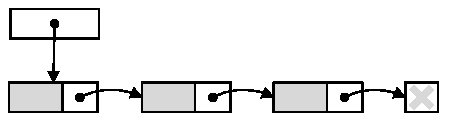
\includegraphics[width=\textwidth]{figures/collections/sll}
				\caption{Singly linked list}
				\label{sll}
			\end{minipage}
			\hspace{0.5cm}
			\begin{minipage}[b]{0.45\linewidth}
				\centering
				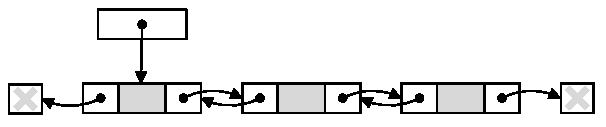
\includegraphics[width=\textwidth]{figures/collections/dll}
				\caption{Doubly linked list}
				\label{dll}
			\end{minipage}
		\end{figure}
		\begin{figure}[h]
			\centering
			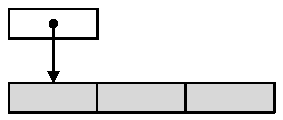
\includegraphics{figures/collections/list}
			\caption{Dynamic array or list structure}
			\label{list}
		\end{figure}
		
		A variable number of nodes is implemented in an AST by nesting container nodes up to the depth required, forming either a singly or doubly linked list (resp. \cref{sll} and \cref{dll}). A node holding any number of child nodes might be represented in \cs as in snippet \cref{col-sample}.

		\begin{codebox}[label=col-sample]{Example of lists as traversible attributes}
			\csharpfile{samples/lists_as_attribs.cs}
		\end{codebox}
	
		This poses the question how such a list property should be handled. 
		
		Case with collections:
		- Node child may be node (or derived) or list of nodes
		- Discriminated union in C\# (https://stackoverflow.com/questions/3151702/discriminated-union-in-c-sharp)
		- What doesn't work: Every node is also a list of nodes
		- Cyclic dependency in inheritance (Node : IList?)
		- Advantages: easy to add, iterate and replace
		- Disadvantages: Traversal issues (can a handler return a list?), complicates everything
		
		Case without collections:
		- More natural to traversals
		- Singly-linked or doubly-linked
		- Difficult to append to or modify
		- Can be overcome with extension methods
		
		Outcome: chosen for no collection types in lists, to avoid confusion with traversals.
		
	

\chapter{Usability And Maintainance Comparison}
	Ranking two different software packages is inherently subjective, though such an approach is actually warranted in this situation. The \cs framework has been field tested by one group from the 2015 course, who managed to deliver a compiler with all optional features earning them one of the highest grades in the class. This proves at the very least that the \cs framework can be used for the course.
	
	\section{Usability}
		While the lack of documentation might appear as a major blow to usability, a more pressing issue is found in the organization of the framework. The framework languages are none of those. While the transformations are well documented, the chance of anyone reading them are slim as they are tucked away in the framework directory, which is excluded from any user interaction. An example of this is the relocation of the scan/parse phase implementation file to the framework folder, even though a dedicated folder is available. This adds to the black box that is the build process.
		
		Running \code{make} can be a scary thing. The roughly 300 line \code{Makefile} is grouped by function and spread out over five files and while certainly clarifying where you should add your code, it doesn't make it any more clear how the process actualy works. This is a shame, because the foundations are actually incredibly well laid out. So, it's not the lack of documentation per se, the process is intentionally obscured. One could say the code generation layer is also to blame. It takes 32 XSLT transformations to generate the code necessary for the most basic compiler.
		
			Clarity of user code: conciseness
			
			Transparency of framework (how easy it is to comprehend action)
			
			So, where to start?
			
			
			
			Maintainability (size)
			
			Other features (discussion):
			\begin{itemize}
			\item NuGet support for package updates
			\item ANTLR4? (LL(*) with EBNF). Better libraries might be a point
			\item More relevant examples found with standard lib
			\
			\end{itemize}
		
	
	\section{Maintainability}
		Software maintainability is at least in part affected by size of the code base. Rough figures on code size were collected using the free tool LocMetrics, which computes various source lines of code (SLOC) metrics. Using lines of code for anything other than exploratory research is dangerous, as there is no scientific consensus on what universally qualifies as a line. However, there is some agreement on what is applicable for C-based languages.
		
		When discussing lines of code, a distinction is generally made between the number lines in a file and the logical executable lines of source code (SLOC-L), with a logical line possibly spanning multiple lines. For C-based languages the logically executable lines of code metric is calculated with relative easy by simply summing all terminal semicolons and terminal curly braces\cite{nguyen2007sloc}. However, logical lines of code \emph{excludes} preprocessor directives and considering a sizeable part of C-based framework is in some dependant on macros, a broader definition is necessary. LogMetrics defines the physical executable lines of code (SLOC-P) as all lines in a file, minus blank lines and comment lines. These three metrics combined should give a clear indication on the size of the projects.
		
		One problem in assessing the size of the C-based framework is in the XSLT transformations and generated code. XSLT is a programming language in itself, is Turing complete and should at least in some way be integrated. No SLOC measures are known for XSLT, instead a figure for the raw lines was chosen. The transformation sheets contain some documentation, so 25\% has been deducted from the raw number of lines. Rather than measuring the sum of generated code and the framwork base code, two measures were used: one for the base code without generated code (no-gen), and one for purely the generated code (gen-only).
		
		The \cs framework has a seperate project with unit tests, these have not been included with the reference metrics but are recorded seperately.
				
		\begin{table}[h]
			\centering
			\bgroup
			\def\arraystretch{1.25}
			\begin{tabular}{|ll|c|c|c|c|}
				\hline
				\multicolumn{2}{|l|}{{\it Framework}} & \multicolumn{1}{l|}{{\bf Lines}} & \multicolumn{1}{l|}{{\bf SLOC-P}} & \multicolumn{1}{l|}{{\bf SLOC-L}} & \multicolumn{1}{l|}{{\bf Files}} \\ \hline
				C (*.c; *.h) & {\it no-gen} & 9800 & 3800 & 2200 & 40 \\ \hline
				C (*.c; *.h) & {\it gen-only} & 8500 & 5300 & 2900 & 21 \\ \hline
				\multicolumn{2}{|l|}{C (*.xsl)} & 5000 & N/A & N/A & 32 \\ \hline
				\multicolumn{2}{|l|}{\cs (*.cs)} & 1350 & 980 & 560 & 19 \\ \hline
				\cs (*.cs) & {\it unit tests} & 830 & 620 & 355 & 10 \\ \hline
			\end{tabular}
			\egroup
			\caption{Framework size metrics}
			\label{locmetrics}
		\end{table}
		
		\begin{comment}
		\begin{table}[h]
			\centering
			\bgroup
			\def\arraystretch{1.25}
			\begin{tabular}{r|c|c|c|c|}
				\cline{2-5}
				\multicolumn{1}{c|}{} & {\bf \begin{tabular}[c]{@{}c@{}}Framework\\ .c \& .h\\ (no-gen)\end{tabular}} & {\bf \begin{tabular}[c]{@{}c@{}}Framework\\ .c \& .h\\ (gen-only)\end{tabular}} & {\bf \begin{tabular}[c]{@{}c@{}}User code\\ .c \& .h\end{tabular}} & {\bf \begin{tabular}[c]{@{}c@{}}XSLT\\ transformations\end{tabular}} \\ \hline
				\multicolumn{1}{|r|}{{\it Lines}} & 9800 & 8500 & 4000 & 6600 \\ \hline
				\multicolumn{1}{|r|}{{\it SLOC (physical)}} & 3800 & 5300 & 2800 & N/A \\ \hline
				\multicolumn{1}{|r|}{{\it SLOC (logical)}} & 2200 & 2900 & 2000 & N/A \\ \hline
				\multicolumn{1}{|r|}{{\it Comment lines}} & 4200 & 2700 & 300 & N/A \\ \hline
				\multicolumn{1}{|r|}{{\it File count}} & 40 & 21 & 33 & 32 \\ \hline
			\end{tabular}
			\egroup
			\caption{Framework and user code size estimates (n=1)}
		\end{table}
		
		\begin{table}[h]
			\centering
			\bgroup
			\def\arraystretch{1.25}
			\begin{tabular}{r|c|c|}
				\cline{2-3}
				& {\bf Lines} & {\bf Size (KB)} \\ \hline
				\multicolumn{1}{|r|}{{\it Average}} & 1300 & 40 \\ \hline
				\multicolumn{1}{|r|}{{\it Minimum}} & 1271 & 31 \\ \hline
				\multicolumn{1}{|r|}{{\it Maximum}} & 1760 & 49 \\ \hline
			\end{tabular}
			\egroup
			\caption{Measurements on the size of the XML specification (n=9)}
			\label{astsize}
		\end{table}
		
		\subsubsection{Observations}
		\paragraph{Full-feature compiler has less code than framework}
		The base library excluding generated code and transformations is equal in complexity to all user travesals combined. 
		
		\paragraph{Framework code is sparsely distributed}
		This cannot be truly said without more data.
		
		\paragraph{XML specification unmaintainable}
		All negatives here:
		
		Large size makes it difficult and uninviting to modify AST structure (40KB to specify a 24 nodes and some traversals)
		
		Abstraction layer is leaky: changing order of child nodes causes reordering in create routine, difficult to notice.
		
		Friendly names for types are not fully implemented.
		
		
	\section{Maintainability}
		XSLT portion nearly equal in size to C portion (rough guess), and nobody likes XSLT: who will support it?
		
		Enough measures in place to judge AST (graph, doc), in-depth code analysis impossible
		
		Maintainability is pretty boring, merge with usability?
		
		Bug: TRAVcont doesn't check for null, will cause dump
		
		
		\section{Strengths And Weaknesses}
		This section will provide an overview of strengths and weaknesses of the framework. A short analysis on the used languages will be made, followed by a summation of framework characteristics grouped under directly affected by language or directly affected by design. Two sections near the end provide insight into the maintainability and ease-of-use for the framework.
		
		Before immediately dilluting the line between language characteristic and design choice, let's consider C as a language. The primary benefits of C are performance, relatively simple syntax and weak typing. These exact points are also the main drawbacks. To clarify, C provides the toolset necessary to craft compact, highly-optimized and efficient code for almost every platform. The simplicity of the language greatly increases the transparency with respect to the resulting assembly and weak typing allows pointer arithmetic not found in most languages. The fast inverse square root\cite{wong1998method} party responsible for the success of the Quake-III game engine is an example of an optimization which is easily added to a C project, but impossible to add to higher languages without modifications to a compiler.
		
		In exchange for this extreme level of control it lacks many luxuries found in modern languages, such as automatic memory management, garbage collection, exceptions, strong and static typing, runtime checks, reflection, object inheritance or composition, to name a few. While some argue that C can be an object-oriented language\cite{book:schreiner}, working with C will always require defensive programming and dynamic typecasts to achieve what modern languages get for free. The group of programmers who should care about low-level instructions is getting smaller every year, continue this rant? Perhaps discussion.
		
		The use of XSLT as a transformation language makes sense considering it's the only platform independent way to transform a specification into something else without resorting to a custom domain specific language (DSL), which requires another compiler. XSLT is turing complete, but programming it is not a challenge most users are interested in. The verbose syntax and templated approach result in code which is spread out, hard to understand and difficult to debug.
		
		\subsubsection{Areas negatively influenced by languages}
		\paragraph{Allocation statements and free traversal}
		A managed language with garbage collection removes the need for a free traversal entirely, and while initiazation code is most always necessary, it will likely be much more compact and less error prone.
		
		\paragraph{Types in validation traversal}
		As explained in \cref{tree-validation}, C is a weakly typed language and any node is a valid AST unless externally validated. A similar approach could be employed by any language, however it is likely a strongly typed language with an some OO-features is able to provide more protection.
		
		\paragraph{Redundancy in traversals declarations}
		In C, definition is always seperated from implementation with header and source files. While this is a useful construct, everything in the compiler framework is declared on the global scope and inter-connected which takes away from the usefulness of definitions. Another form of redundancy is found in the configuration of the pipline and traversal specification. Though identified as two distinct regions, it is unlikely users will write many traversals outside of the ones directly called from the pipeline.
		
		\paragraph{Verbosity and size of specification file}
		Though simple in concept, the \code{AST.xml} file quickly grows for even relatively simple compilers. 
		
		\paragraph{Tracer statements}
		A minor nuisance to some, the plethora of \code{DBUG\_ENTER} and \code{DBUG\_EXIT} tags mixed in all code eliminates compact code. The command line support permitting these was so rarely used none of the course instructors knew how to enable it.
		
		\subsubsection{Positive design decisions}
		\paragraph{Traversal mechanism}
		There are not many ways to go about changing an AST, but the enormous potential in the traversal mechanism is not hard to spot. It enforces a clean seperation of structure and algorithm and groups related tasks into logical components. While the creation of a \emph{god}-traversal spanning thousands of line is not uncommon, this is most likely due to the difficulty with setting them up. The approach actually dictates realization of small, re-usable blocks for the rest of the compiler.
		
		\paragraph{Phase-based transformations}
		While most compiler frontends employ some form of sequential processing, the decision to integrate AST traversals directly into a configurable pipeline is elegant and serves it's purpose very well. It imposes a structured way to think about the compilation process, without exceptions down the line.
		
		\paragraph{Phase range in validation traversal}
		Though it has limited use in smaller compilers, the feature itself embodies a powerful concept: that of a changing AST.
		
		\end{comment}


\chapter{Discussion}

	Nope.
	\begin{comment}
	Polyglot: if it provides suitable routines, it is well maintained and might be a better option.

	\section{Language Quotes}
		Static typing a source of documentation\cite{Hanenberg2014}
		
		Static typing may not be helpful in preventing semantic errors\cite{Hanenberg2014}
		
		Static type systems help humans use a new set of classes\cite{Hanenberg2014}
		
		Nanz:
		C is hard to beat when it comes to raw speed on large inputs,
		compiled strongly-typed languages,
		where more defects can be caught at compile time, are less prone
		to runtime failures than interpreted or weakly-typed languages
		vNext immutable AST, 
		
		Language choice, developers switch language often
			We found that developers rapidly and frequently learn
			languages. Factors such as age play a smaller role than suggested
			by media. In contrast, which languages developers
			learn is influenced by their education, and in particular, curriculum
			design.
			
		Functional
			Promisingly, developers who learned a functional or	math-oriented language in school are more than twice as likely to know one later than those who did not.
	
	\section{Language Selection}
		While C is arguably as modern and widely used as any other general purpose programming language, and can even be called object-oriented \cite{book:schreiner}, it is definiatly not strongly typed. Programming in C requires defensive programming and dynamic type casts to achieve a level of safety other languages get for free, as internally every structure is a \code{void*}. In this section the language options for a modernized Civic framework are briefly discussed.
		
		Choosing a language is a non-trivial task and depends on many factors. For this project, the first criteria was that the language must be high-level and preferably managed to reduce the time spent debugging memory allocation and null references in C. Student familiarity with the language was also considered, as well as the exclusion of any fully functional languages. The reason for the latter being removal of the functional programming course from the undergraduate program. One final consideration was the availability of relevant libraries and support infrastructure. 
		
		With functional languages excluded, procedural and scripting languages remain. A recent study found the most common languages on GitHub in these categories to be C++, C\#, Objective-C, Java, Go, JavaScript, Python, Perl, Php and Ruby \cite{Ray2014}. A study by \citeauthor{Meyerovich2013} found that 97\% of computer science majors knew at least one imperative/OO language against 78\% for dynamic languages \cite{Meyerovich2013}. Studies on static versus dynamic typing are somewhat inconclusive, though evidence suggests static typing improves maintainability, increases understanding of undocumented code and measurably reduces defects \cite{Hanenberg2014,Ray2014}.
		
		When considering only statically typed managed languages, only C\#, Java and Go remain. The TIOBE index is a  programming language popularity index based on the number of hits in various search engines. While Java and C\# occupy position 3 and 6 respectively, Go takes the 30th place, just below Ada \cite{Nanz2014}. With both C\# and Java able to use the LL(*) ANTLR4 parser generator, either of these languages would suit the project.
		
		Todo:
		\begin{itemize}
			\item C\# has more powerful semantics, lambdas, properties, optional dynamic typing
			\item But it is somewhat plaform bound, whereas Java is not
		\end{itemize}
	
	\end{comment}
		

\bibliography{report}
\bibliographystyle{plainnat}
\end{document}